
%% bare_conf.tex
%% V1.3
%% 2007/01/11
%% by Michael Shell
%% See:
%% http://www.michaelshell.org/
%% for current contact information.
%%
%% This is a skeleton file demonstrating the use of IEEEtran.cls
%% (requires IEEEtran.cls version 1.7 or later) with an IEEE conference paper.
%%
%% Support sites:
%% http://www.michaelshell.org/tex/ieeetran/
%% http://www.ctan.org/tex-archive/macros/latex/contrib/IEEEtran/
%% and
%% http://www.ieee.org/

%%*************************************************************************
%% Legal Notice:
%% This code is offered as-is without any warranty either expressed or
%% implied; without even the implied warranty of MERCHANTABILITY or
%% FITNESS FOR A PARTICULAR PURPOSE! 
%% User assumes all risk.
%% In no event shall IEEE or any contributor to this code be liable for
%% any damages or losses, including, but not limited to, incidental,
%% consequential, or any other damages, resulting from the use or misuse
%% of any information contained here.
%%
%% All comments are the opinions of their respective authors and are not
%% necessarily endorsed by the IEEE.
%%
%% This work is distributed under the LaTeX Project Public License (LPPL)
%% ( http://www.latex-project.org/ ) version 1.3, and may be freely used,
%% distributed and modified. A copy of the LPPL, version 1.3, is included
%% in the base LaTeX documentation of all distributions of LaTeX released
%% 2003/12/01 or later.
%% Retain all contribution notices and credits.
%% ** Modified files should be clearly indicated as such, including  **
%% ** renaming them and changing author support contact information. **
%%
%% File list of work: IEEEtran.cls, IEEEtran_HOWTO.pdf, bare_adv.tex,
%%                    bare_conf.tex, bare_jrnl.tex, bare_jrnl_compsoc.tex
%%*************************************************************************

% *** Authors should verify (and, if needed, correct) their LaTeX system  ***
% *** with the testflow diagnostic prior to trusting their LaTeX platform ***
% *** with production work. IEEE's font choices can trigger bugs that do  ***
% *** not appear when using other class files.                            ***
% The testflow support page is at:
% http://www.michaelshell.org/tex/testflow/



% Note that the a4paper option is mainly intended so that authors in
% countries using A4 can easily print to A4 and see how their papers will
% look in print - the typesetting of the document will not typically be
% affected with changes in paper size (but the bottom and side margins will).
% Use the testflow package mentioned above to verify correct handling of
% both paper sizes by the user's LaTeX system.
%
% Also note that the "draftcls" or "draftclsnofoot", not "draft", option
% should be used if it is desired that the figures are to be displayed in
% draft mode.
%
\documentclass[10pt, conference, compsocconf]{IEEEtran}
% Add the compsocconf option for Computer Society conferences.
%
% If IEEEtran.cls has not been installed into the LaTeX system files,
% manually specify the path to it like:
% \documentclass[conference]{../sty/IEEEtran}





% Some very useful LaTeX packages include:
% (uncomment the ones you want to load)


% *** MISC UTILITY PACKAGES ***
%
%\usepackage{ifpdf}
% Heiko Oberdiek's ifpdf.sty is very useful if you need conditional
% compilation based on whether the output is pdf or dvi.
% usage:
% \ifpdf
%   % pdf code
% \else
%   % dvi code
% \fi
% The latest version of ifpdf.sty can be obtained from:
% http://www.ctan.org/tex-archive/macros/latex/contrib/oberdiek/
% Also, note that IEEEtran.cls V1.7 and later provides a builtin
% \ifCLASSINFOpdf conditional that works the same way.
% When switching from latex to pdflatex and vice-versa, the compiler may
% have to be run twice to clear warning/error messages.






% *** CITATION PACKAGES ***
%
\usepackage{cite}
% cite.sty was written by Donald Arseneau
% V1.6 and later of IEEEtran pre-defines the format of the cite.sty package
% \cite{} output to follow that of IEEE. Loading the cite package will
% result in citation numbers being automatically sorted and properly
% "compressed/ranged". e.g., [1], [9], [2], [7], [5], [6] without using
% cite.sty will become [1], [2], [5]--[7], [9] using cite.sty. cite.sty's
% \cite will automatically add leading space, if needed. Use cite.sty's
% noadjust option (cite.sty V3.8 and later) if you want to turn this off.
% cite.sty is already installed on most LaTeX systems. Be sure and use
% version 4.0 (2003-05-27) and later if using hyperref.sty. cite.sty does
% not currently provide for hyperlinked citations.
% The latest version can be obtained at:
% http://www.ctan.org/tex-archive/macros/latex/contrib/cite/
% The documentation is contained in the cite.sty file itself.






% *** GRAPHICS RELATED PACKAGES ***
%
\ifCLASSINFOpdf
   \usepackage[pdftex]{graphicx}
  % declare the path(s) where your graphic files are
  % \graphicspath{{../pdf/}{../jpeg/}}
  % and their extensions so you won't have to specify these with
  % every instance of \includegraphics
  % \DeclareGraphicsExtensions{.pdf,.jpeg,.png}
\else
  % or other class option (dvipsone, dvipdf, if not using dvips). graphicx
  % will default to the driver specified in the system graphics.cfg if no
  % driver is specified.
  % \usepackage[dvips]{graphicx}
  % declare the path(s) where your graphic files are
  % \graphicspath{{../eps/}}
  % and their extensions so you won't have to specify these with
  % every instance of \includegraphics
  % \DeclareGraphicsExtensions{.eps}
\fi
% graphicx was written by David Carlisle and Sebastian Rahtz. It is
% required if you want graphics, photos, etc. graphicx.sty is already
% installed on most LaTeX systems. The latest version and documentation can
% be obtained at: 
% http://www.ctan.org/tex-archive/macros/latex/required/graphics/
% Another good source of documentation is "Using Imported Graphics in
% LaTeX2e" by Keith Reckdahl which can be found as epslatex.ps or
% epslatex.pdf at: http://www.ctan.org/tex-archive/info/
%
% latex, and pdflatex in dvi mode, support graphics in encapsulated
% postscript (.eps) format. pdflatex in pdf mode supports graphics
% in .pdf, .jpeg, .png and .mps (metapost) formats. Users should ensure
% that all non-photo figures use a vector format (.eps, .pdf, .mps) and
% not a bitmapped formats (.jpeg, .png). IEEE frowns on bitmapped formats
% which can result in "jaggedy"/blurry rendering of lines and letters as
% well as large increases in file sizes.
%
% You can find documentation about the pdfTeX application at:
% http://www.tug.org/applications/pdftex





% *** MATH PACKAGES ***
%
\usepackage[cmex10]{amsmath}
% A popular package from the American Mathematical Society that provides
% many useful and powerful commands for dealing with mathematics. If using
% it, be sure to load this package with the cmex10 option to ensure that
% only type 1 fonts will utilized at all point sizes. Without this option,
% it is possible that some math symbols, particularly those within
% footnotes, will be rendered in bitmap form which will result in a
% document that can not be IEEE Xplore compliant!
%
% Also, note that the amsmath package sets \interdisplaylinepenalty to 10000
% thus preventing page breaks from occurring within multiline equations. Use:
%\interdisplaylinepenalty=2500
% after loading amsmath to restore such page breaks as IEEEtran.cls normally
% does. amsmath.sty is already installed on most LaTeX systems. The latest
% version and documentation can be obtained at:
% http://www.ctan.org/tex-archive/macros/latex/required/amslatex/math/





% *** SPECIALIZED LIST PACKAGES ***
%
%\usepackage{algorithmic}
% algorithmic.sty was written by Peter Williams and Rogerio Brito.
% This package provides an algorithmic environment fo describing algorithms.
% You can use the algorithmic environment in-text or within a figure
% environment to provide for a floating algorithm. Do NOT use the algorithm
% floating environment provided by algorithm.sty (by the same authors) or
% algorithm2e.sty (by Christophe Fiorio) as IEEE does not use dedicated
% algorithm float types and packages that provide these will not provide
% correct IEEE style captions. The latest version and documentation of
% algorithmic.sty can be obtained at:
% http://www.ctan.org/tex-archive/macros/latex/contrib/algorithms/
% There is also a support site at:
% http://algorithms.berlios.de/index.html
% Also of interest may be the (relatively newer and more customizable)
% algorithmicx.sty package by Szasz Janos:
% http://www.ctan.org/tex-archive/macros/latex/contrib/algorithmicx/




% *** ALIGNMENT PACKAGES ***
%
%\usepackage{array}
% Frank Mittelbach's and David Carlisle's array.sty patches and improves
% the standard LaTeX2e array and tabular environments to provide better
% appearance and additional user controls. As the default LaTeX2e table
% generation code is lacking to the point of almost being broken with
% respect to the quality of the end results, all users are strongly
% advised to use an enhanced (at the very least that provided by array.sty)
% set of table tools. array.sty is already installed on most systems. The
% latest version and documentation can be obtained at:
% http://www.ctan.org/tex-archive/macros/latex/required/tools/


%\usepackage{mdwmath}
%\usepackage{mdwtab}
% Also highly recommended is Mark Wooding's extremely powerful MDW tools,
% especially mdwmath.sty and mdwtab.sty which are used to format equations
% and tables, respectively. The MDWtools set is already installed on most
% LaTeX systems. The lastest version and documentation is available at:
% http://www.ctan.org/tex-archive/macros/latex/contrib/mdwtools/


% IEEEtran contains the IEEEeqnarray family of commands that can be used to
% generate multiline equations as well as matrices, tables, etc., of high
% quality.


\usepackage{eqparbox}
% Also of notable interest is Scott Pakin's eqparbox package for creating
% (automatically sized) equal width boxes - aka "natural width parboxes".
% Available at:
% http://www.ctan.org/tex-archive/macros/latex/contrib/eqparbox/





% *** SUBFIGURE PACKAGES ***
\usepackage[tight,footnotesize]{subfigure}
% subfigure.sty was written by Steven Douglas Cochran. This package makes it
% easy to put subfigures in your figures. e.g., "Figure 1a and 1b". For IEEE
% work, it is a good idea to load it with the tight package option to reduce
% the amount of white space around the subfigures. subfigure.sty is already
% installed on most LaTeX systems. The latest version and documentation can
% be obtained at:
% http://www.ctan.org/tex-archive/obsolete/macros/latex/contrib/subfigure/
% subfigure.sty has been superceeded by subfig.sty.



%\usepackage[caption=false]{caption}
%\usepackage[font=footnotesize]{subfig}
% subfig.sty, also written by Steven Douglas Cochran, is the modern
% replacement for subfigure.sty. However, subfig.sty requires and
% automatically loads Axel Sommerfeldt's caption.sty which will override
% IEEEtran.cls handling of captions and this will result in nonIEEE style
% figure/table captions. To prevent this problem, be sure and preload
% caption.sty with its "caption=false" package option. This is will preserve
% IEEEtran.cls handing of captions. Version 1.3 (2005/06/28) and later 
% (recommended due to many improvements over 1.2) of subfig.sty supports
% the caption=false option directly:
%\usepackage[caption=false,font=footnotesize]{subfig}
%
% The latest version and documentation can be obtained at:
% http://www.ctan.org/tex-archive/macros/latex/contrib/subfig/
% The latest version and documentation of caption.sty can be obtained at:
% http://www.ctan.org/tex-archive/macros/latex/contrib/caption/




% *** FLOAT PACKAGES ***
%
%\usepackage{fixltx2e}
% fixltx2e, the successor to the earlier fix2col.sty, was written by
% Frank Mittelbach and David Carlisle. This package corrects a few problems
% in the LaTeX2e kernel, the most notable of which is that in current
% LaTeX2e releases, the ordering of single and double column floats is not
% guaranteed to be preserved. Thus, an unpatched LaTeX2e can allow a
% single column figure to be placed prior to an earlier double column
% figure. The latest version and documentation can be found at:
% http://www.ctan.org/tex-archive/macros/latex/base/



\usepackage{stfloats}
% stfloats.sty was written by Sigitas Tolusis. This package gives LaTeX2e
% the ability to do double column floats at the bottom of the page as well
% as the top. (e.g., "\begin{figure*}[!b]" is not normally possible in
% LaTeX2e). It also provides a command:
%\fnbelowfloat
% to enable the placement of footnotes below bottom floats (the standard
% LaTeX2e kernel puts them above bottom floats). This is an invasive package
% which rewrites many portions of the LaTeX2e float routines. It may not work
% with other packages that modify the LaTeX2e float routines. The latest
% version and documentation can be obtained at:
% http://www.ctan.org/tex-archive/macros/latex/contrib/sttools/
% Documentation is contained in the stfloats.sty comments as well as in the
% presfull.pdf file. Do not use the stfloats baselinefloat ability as IEEE
% does not allow \baselineskip to stretch. Authors submitting work to the
% IEEE should note that IEEE rarely uses double column equations and
% that authors should try to avoid such use. Do not be tempted to use the
% cuted.sty or midfloat.sty packages (also by Sigitas Tolusis) as IEEE does
% not format its papers in such ways.





% *** PDF, URL AND HYPERLINK PACKAGES ***
%
\usepackage{url}
% url.sty was written by Donald Arseneau. It provides better support for
% handling and breaking URLs. url.sty is already installed on most LaTeX
% systems. The latest version can be obtained at:
% http://www.ctan.org/tex-archive/macros/latex/contrib/misc/
% Read the url.sty source comments for usage information. Basically,
% \url{my_url_here}.





% *** Do not adjust lengths that control margins, column widths, etc. ***
% *** Do not use packages that alter fonts (such as pslatex).         ***
% There should be no need to do such things with IEEEtran.cls V1.6 and later.
% (Unless specifically asked to do so by the journal or conference you plan
% to submit to, of course. )


% correct bad hyphenation here
\hyphenation{op-tical net-works semi-conduc-tor}


\begin{document}
%
% paper title
% can use linebreaks \\ within to get better formatting as desired
\title{Defining NUMA Affinity for OpenMP Threads}


% author names and affiliations
% use a multiple column layout for up to two different
% affiliations

\author{\IEEEauthorblockN{Swaroop Pophale, Oscar Hernandez}
\IEEEauthorblockA{Computer Science and Mathematics Division \\
ORNL\\
Oak Ridge, USA\\
{pophaless, oscar}@ornl.gov}
%\and
%\IEEEauthorblockN{Authors Name/s per 2nd Affiliation (Author)}
%\IEEEauthorblockA{line 1 (of Affiliation): dept. name of organization\\
%line 2: name of organization, acronyms acceptable\\
%line 3: City, Country\\
%line 4: Email: name@xyz.com}
}

% conference papers do not typically use \thanks and this command
% is locked out in conference mode. If really needed, such as for
% the acknowledgment of grants, issue a \IEEEoverridecommandlockouts
% after \documentclass

% for over three affiliations, or if they all won't fit within the width
% of the page, use this alternative format:
% 
%\author{\IEEEauthorblockN{Michael Shell\IEEEauthorrefmark{1},
%Homer Simpson\IEEEauthorrefmark{2},
%James Kirk\IEEEauthorrefmark{3}, 
%Montgomery Scott\IEEEauthorrefmark{3} and
%Eldon Tyrell\IEEEauthorrefmark{4}}
%\IEEEauthorblockA{\IEEEauthorrefmark{1}School of Electrical and Computer Engineering\\
%Georgia Institute of Technology,
%Atlanta, Georgia 30332--0250\\ Email: see http://www.michaelshell.org/contact.html}
%\IEEEauthorblockA{\IEEEauthorrefmark{2}Twentieth Century Fox, Springfield, USA\\
%Email: homer@thesimpsons.com}
%\IEEEauthorblockA{\IEEEauthorrefmark{3}Starfleet Academy, San Francisco, California 96678-2391\\
%Telephone: (800) 555--1212, Fax: (888) 555--1212}
%\IEEEauthorblockA{\IEEEauthorrefmark{4}Tyrell Inc., 123 Replicant Street, Los Angeles, California 90210--4321}}




% use for special paper notices
%\IEEEspecialpapernotice{(Invited Paper)}
% make the title area
\maketitle


\begin{abstract}
%The abstract goes here. DO NOT USE SPECIAL CHARACTERS, SYMBOLS, OR MATH IN YOUR TITLE OR ABSTRACT.


%OLD 
%As we move toward pre-Exascale systems, two of the DOE leadership class systems will consist of very powerful OpenPOWER compute nodes which will be more complex to program. These systems will have massive amounts of parallelism; where threads may be running on POWER9 cores as well as on accelerators. Advances in memory interconnects, such as NVLINK, will provide a unified shared memory address spaces for different types of memories HBM, DRAM, etc. In preparation for such system, we need to improve our understanding on how OpenMP supports the concept of affinity as well as memory placement on POWER8 systems. Data locality and affinity are key program optimizations to exploit the compute and memory capabilities to achieve good performance by minimizing data motion across NUMA domains and access the cache efficiently. This paper is the first step to evaluate the current features of OpenMP 4.0 on the POWER8 processors, and on how to measure its effects on a system with two POWER8 sockets. We experiment with the different affinity settings provided by OpenMP 4.0 to quantify the costs of having good data locality vs not,  and measure their effects via hardware counters. We also find out which affinity settings benefits more from data locality. Based on this study we describe the current state of art, the challenges we faced in quantifying effects of affinity, and and ideas on how OpenMP 5.0 should be improved to address affinity in the context of NUMA domains and accelerators.


\let\thefootnote\relax\footnote{This manuscript has been authored by UT-Battelle, LLC under Contract No. DE-AC05-00OR22725 with the U.S. Department of Energy. The United States Government retains and the publisher, by accepting the article for publication, acknowledges that the United States Government retains a non-exclusive, paid-up, irrevocable, worldwide license to publish or reproduce the published form of this manuscript, or allow others to do so, for United States Government purposes. The Department of Energy will provide public access to these results of federally sponsored research in accordance with the DOE Public Access Plan (http://energy.gov/downloads/doe-public-access-plan).}

\end{abstract}

\begin{IEEEkeywords}
component; formatting; style; styling;

\end{IEEEkeywords}


% For peer review papers, you can put extra information on the cover
% page as needed:
% \ifCLASSOPTIONpeerreview
% \begin{center} \bfseries EDICS Category: 3-BBND \end{center}
% \fi
%
% For peerreview papers, this IEEEtran command inserts a page break and
% creates the second title. It will be ignored for other modes.
\IEEEpeerreviewmaketitle

\section{Introduction}
% How affinity works on 4.0 and 4.5
% What discussions are being proposed for 5.0 --telecon
\label{sec:intro}
%The effects of affinity is a widely studied problem. Most programming models 
take advantage of the architecture and data-access patterns by providing some 
implicit or explicit mechanism to control data and process/thread placement. For example,
Partitioned Global Address Space (PGAS) languages/APIs provide mechanisms to specify 
globally accessible data (with local views) that can be distributed to a thread local memory (affine memory). 
Unified Parallel C, a PGAS language, provides a \textbf{shared} qualifier to distinguish between data 
accessible to all the UPC \textit{threads} vs. private data and distribution keywords to place
the data on different affine memories. For arrays UPC provides 
three affinity granularities: blocked, cyclic and blocked-cyclic. In addition to these
UPC provides an affinity field in \textbf{upc\_forall} to schedule loop iterations to threads with local data.
(A similar affinity concept~\cite{nikolopoulos2001exploiting} has been proposed as an extension to the schedule clause in the OpenMP \textbf{parallel for} construct).
%The \textit{shared} scalar data has 
%affinity to thread 0, while arrays can have affinity granularity of \textit{cyclic, blocked-cyclic ,}
%and \textit{blocked}. These are chosen by the application programmer based on the 
%knowledge of the data access patterns within the application. 

OpenMP 4.0 being a shared memory programming model, it has 
different ways to control (implicit and explicitly) the affinity of data (first touch policy, privatization, etc), threads, and the mapping of work to threads.
work-sharing constructs. OpenMP 4.0 also provides a mechanism to map data to and from accelerators using \textit{target data} regions. The new OpenMP 4.5 release provides a substantial 
improvement on the support for programming of accelerator and GPU devices and to control
how data is being mapped to/from a target device by unstructured data regions and a new \textit{firstprivate} default for scalars.
%Amongst the new features introduced are, support for parallelization of loops with 
%well-structured dependencies, mechanisms for unstructured data mapping and 
%asynchronous execution, support to divide loops into tasks without requiring all 
%threads to execute the loop, reductions for C/C++ arrays, a new hint mechanisms to 
%provide guidance on the relative priority of tasks and on preferred synchronization 
%implementations, SIMD extensions, improved support for Fortran 2003, and
%thread affinity support through runtime functions to determine the effect of thread 
%affinity clauses. In this paper we focus on the affinity aspect of OpenMP with respect 
%to the emerging OpenPOWER systems.

\subsection{Memory Placement}
Most systems provide implicit data placement control through policies like \textit{first-touch} 
and \textit{next-touch}. First-touch is more appropriate for applications where the 
first access to data is representative of the application\'s data accesses throughout 
the life of the application. This policy has been adopted as default on many systems. 
For applications that have a more dynamic access pattern, the \textit{next-touch} 
policy may be more appropriate. Here the data is marked to be placed on the node of the 
next CPU that accesses it. For OpenMP, \textit{first-touch} translates to data being 
placed near the thread that first accesses it. Even without any other affinity mechanism this 
can cause significant impact, for e.g., if the data is initialized by thread 0 only, but later is accessed 
by all the threads, the \textit{first-touch} policy would locate memory on the node where 
thread 0 is placed thus resulting in remote memory accesses costs for threads not placed on the same node. 

\subsection{Thread Affinity}
OpenMP 4.5 provides OMP\_PROC\_BIND ICV to set the thread affinity policy. The legitimate value for 
this environment variable is either true, false, or a comma separated list of master, close, or spread. 
When the values are specified in a list, they correspond to the thread affinity policy to be used for 
parallel regions at the corresponding nested level. In combination with the OMP\_PLACES ICV, 
users may have complete control on the thread affinity and their placement on a given hardware. 
OMP\_PLACES ICV can be one of two types of values: either an abstract name describing a set 
of places or an explicit list of places described by non-negative numbers. Pre-defined abstract 
names include \textit{threads, cores,} and \textit{sockets}. A hardware thread is the smallest execution 
unit that a thread can be bound to with OpenMP 4.5. 


When expressed as numbers, places 
represent the smallest unit of execution exposed by the execution environment, which is typically 
a hardware thread. In conjunction to places represented by non-negative numbers, intervals is another handy way to 
express \textit{places} in OpenMP. They are specified using the \textit{$<$lower-bound$>$ : $<$length$>$ : $<$stride$>$} notation. For example, a user could specify exact cores to place the OpenMP threads or a range of cores based on the application characteristics to best utilize the underlying hardware.

%For example; setenv OMP\_PLACES threads, setenv OMP\_PLACES ``threads(2)", setenv OMP\_PLACES ``{0, 1, 2, 3}, {4, 5, 6, 7}", setenv OMP\_PLACES ``{0:4}, {4:4}, {8:4}, {12:4}", and setenv OMP\_PLACES ``{0:4}:4:4" are equivalent and will result in the binding of OpenMP threads to sixteen consecutive hardware threads. 

\subsection{POWER8 System}

The POWER8 processor is a RISC (Reduced Instruction Set Computer) microprocessor from IBM and the first processor supporting the new OpenPOWER eco-system. 
The POWER8 processor has three possible configurations of either 6, 10 or 12 cores per processor chip. Each processor contains two chiplets of 3, 5 or 6 cores.  A typical 12 core processor, as shown in Figure~\ref{fig:p8_1} has  512 KB SRAM L2 caches per core, 96 MB eDRAM shared L3 and an off chip L4 cache that provides up to 128 MB eDRAM space. The L4 cache is supported via an external Centaur memory buffer chip. The Centaur chip is connected via a high-speed link to the POWER8 processor, eDRAM, DDR interfaces, and control logic.This is shown in Figure~\ref{fig:p8_2}. 

\begin{figure}[h!]
  \centering
  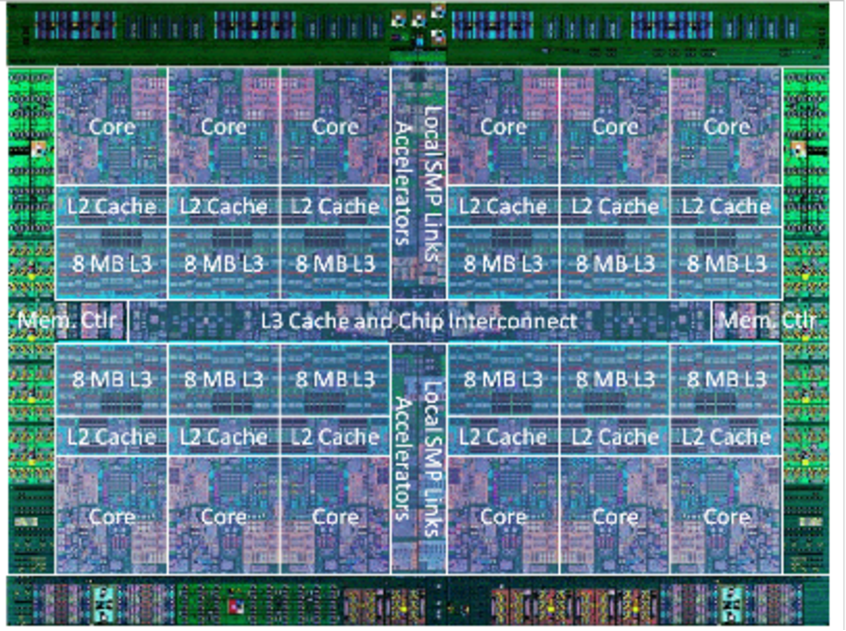
\includegraphics[height=0.4\textwidth, width=0.7\textwidth]{./Images/P8.pdf}
       \caption{IBM POWER8 processor architecture~\cite{IBM_P8}.}
       \label{fig:p8_1}
\end{figure}

\begin{figure}[h!]
  \centering
  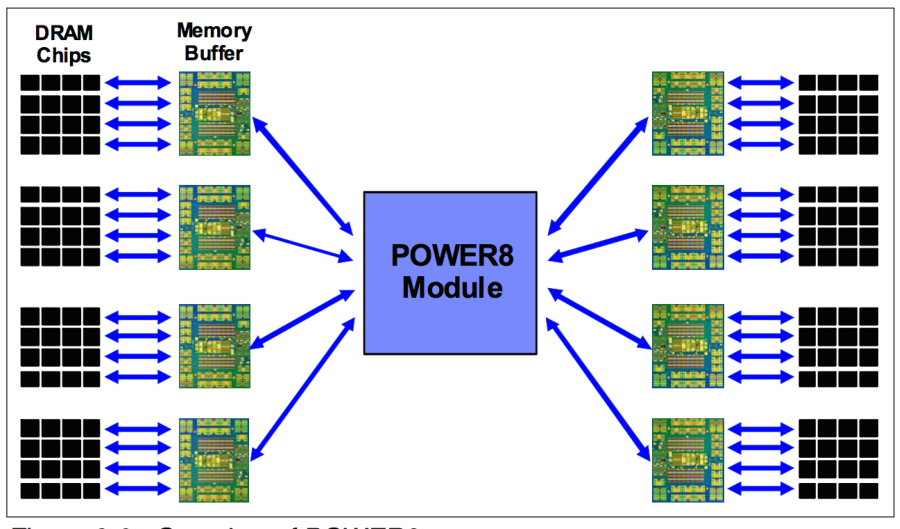
\includegraphics[height=0.4\textwidth, width=0.8\textwidth]{./Images/P8_memory.pdf}
       \caption{IBM POWER8 memory subsystem~\cite{IBM_P8}.}
       \label{fig:p8_2}
\end{figure}
%\begin{figure}
%    \centering
%    \begin{subfigure}[b]{0.4\textwidth}
%         {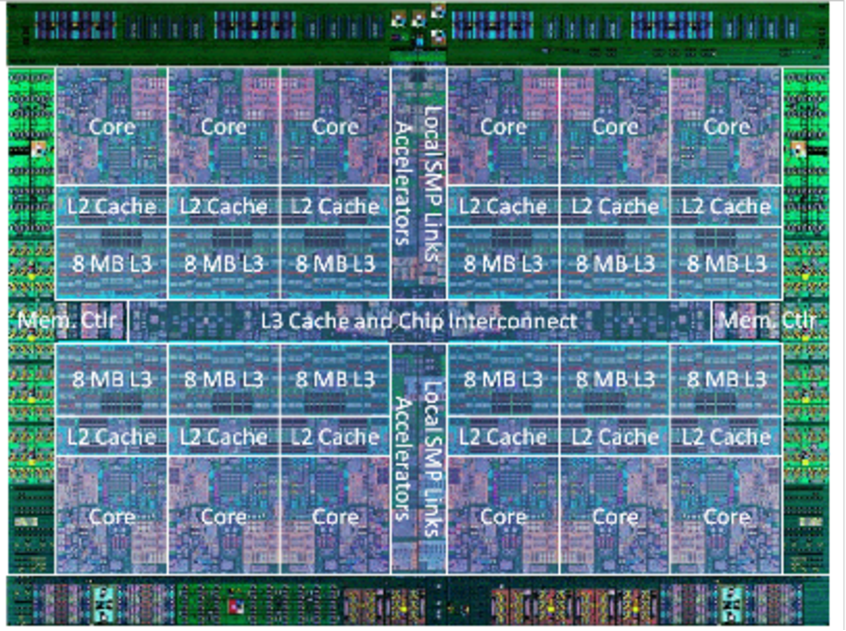
\includegraphics[width=1.0\textwidth]{./Images/P8.pdf}}
%%  	\vspace{-0.0pc}
%	 \caption{POWER8 block diagram.~\cite{IBM_P8}}
% 	 \label{fig:p8_1}
%    \end{subfigure}
%     \centering
%    \begin{subfigure}[b]{0.4\textwidth}
%         {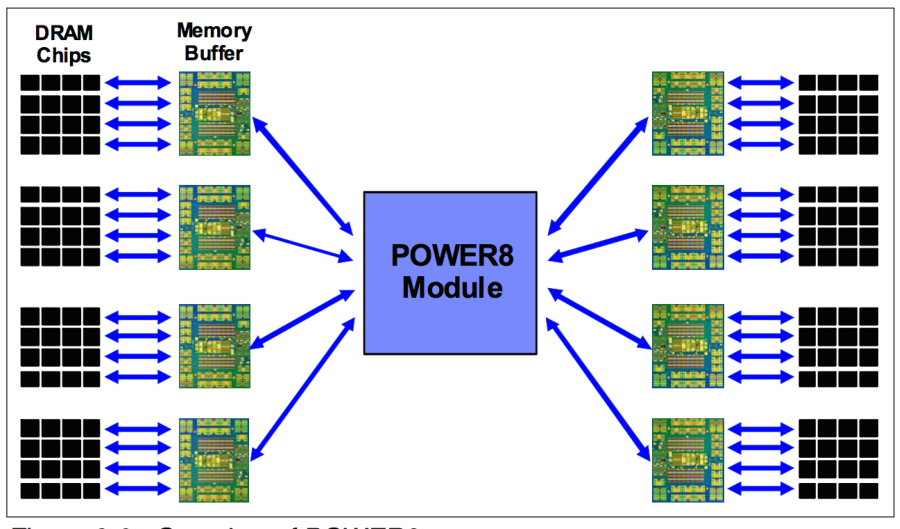
\includegraphics[height=0.7\textwidth]{./Images/P8_memory.pdf}}
%  %	\vspace{-0.0pc}
%	 \caption{POWER8 Memory Subsystem.~\cite{IBM_P8}}
%	  \label{fig:p8_2}
%    \end{subfigure}
%  \caption{POWER8 Overview}\label{fig:POWER8}
%\end{figure}
%Maybe introduce the concept of Chiplet on the P8. What is a chiplet since it defines a numa domain later on.
The POWER8 processor has a Non-Uniform Cache Architecture (NUCA) Cache Policy within the chip, this allows a shared L3 cache with scalable bandwidth and latency, allowing migration of most used cache lines to the local L2 cache and then to the local L1 cache~\cite{IBM_P8}. This is a big improvement over the POWER7 processor.  

When we run the \textit{numactl} command on a two socket POWER8 system with Ubuntu 14.04, the utility reports four NUMA domains: one domain per each POWER8 chiplet. \textit{numactl}  also reports the NUMA distances between domains, which is the ratio of the latency of accessing  a remote numa node memory and local memory access. Figure ~\ref{fig:crest} shows the values of different NUMA distances on a two socket POWER8 system, that we use for our experimentation, as reported by \textit{numactl}.

\begin{figure}[h]
  \centering
  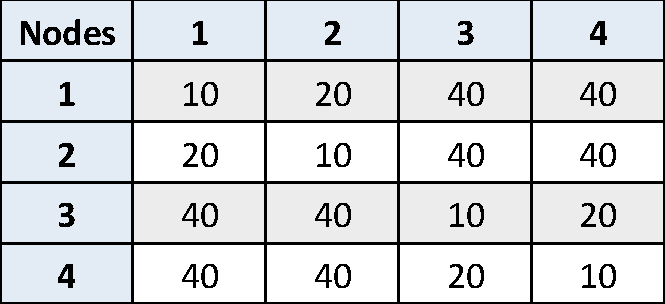
\includegraphics[height=0.25\textwidth]{./Images/crest.pdf}
       \caption{NUMA distances on a two socket POWER8 processor system as reported by \textit{numactl}}
       \label{fig:crest}
\end{figure}

%[4/9/16, 12:37:55 PM] Oscar: we just need to expand the text for that table
%[4/9/16, 12:38:07 PM] Oscar: we need to explain why we have these numbers in blue
%[4/9/16, 12:38:25 PM] Oscar: and why we have these many rows and columns
%[4/9/16, 12:38:38 PM] Oscar: and how that related to a dual socket POWER8 system

\subsection{POWER8 Hardware Counters}
To quantify the effects of data affinity and data locality, we look closely at the different hardware counters available on the POWER8 memory subsystem, including \textbf{data cache} stall cycles. Long cache latencies and cache misses usually indicate poor placement of data with respect to the executing thread in a OpenMP program. Performance instrumentation in POWER8 is provided in two layers: the \textbf{Core Level Performance Monitoring} (CLPM) and the \textbf{Nest Level Performance Monitoring} (NLPM). CLPM allows for monitoring of the core pipeline efficiency of the front-end, branch prediction, schedulers etc., along with behavioral metrics such as stalls, execution rates, thread prioritization and resource sharing, and utilizations of resources etc. On the other hand NLPM provides a way to instrument the L3 cache, interconnect fabric and memory channels/controllers. 
%
\begin{table*}[h]
\vspace{-0.5pc}
\centering
\begin{tabular} { | l | l |}
\hline
%PM\_CMPLU\_STALL\_
*DCACHE\_MISS & Stall by Data Cache (L1) misses\\  \hline
%PM\_CMPLU\_STALL\_
*DMISS\_L2L3 & Stall by Dcache miss which resolved in L2/L3 \\  \hline
%PM\_CMPLU\_STALL\_
*DMISS\_L2L3\_CONFLICT & Stall due to cache miss due to L2 L3 conflict \\  \hline
%PM\_CMPLU\_STALL\_
*DMISS\_L2L3\_NO\_CONFLICT & Stall due to cache miss due to no L2 L3 conflict \\ \hline
%PM\_CMPLU\_STALL\_
*DMISS\_L3MISS & Stall due to cache miss resolving missed the L3 \\ \hline
%PM\_CMPLU\_STALL\_
*DMISS\_LMEM & GCT empty by branch mispredict + IC miss\\ \hline
%PM\_CMPLU\_STALL\_
*DMISS\_L21\_L31 &  Stall by Dcache miss which resolved on chip \\ \hline%(excluding local L2/L3)\\ \hline
%PM\_CMPLU\_STALL\_
*DMISS\_REMOTE  & Stall by Dcache miss which resolved from remote chip \\ \hline%(cache or memory)\\ \hline
%PM\_CMPLU\_STALL\_
*DMISS\_DISTANT & Stall by L1 reloads from distant interventions and memory \\ \hline
 \end{tabular}
 \caption{Explanation of the Data Cache Miss Stall Counters on POWER8 \\ * = PM\_CMPLU\_STALL\_}
\label{tab:hwct}
\end{table*}
%
POWER8 has an enhanced Cycles Per Instruction (CPI) Accounting Model. The POWER8 CPI Stack accounts for stalled, waiting to complete, thread blocked, completion table empty, completion and other miscellaneous cycles. The stalled cycles are further classified based on the cause of the stall. Newly added to this group for the POWER8 architecture is the finer granularity of \textit{Stall cycles due to Dcache Misses}.  Since we want to quantify cycles wasted due to NUCA and NUMA latencies, we focus on the sub-set of hardware counters mentioned in Table~\ref{tab:hwct}. The collection of the counter values are enabled by a system provided script. This allows for access to counters that may not be represented as literal strings and accessible via other application profiling tools. In turn PM\_CMPLU\_STALL\_DCACHE\_MISS and PM\_CMPLU\_STALL\_DMISS\_L3MISS are a summation of stall cycles listed in Table ~\ref{tab:cl}. Although we record all the hardware counter values we only report those that are significantly affected by data affinity.
%
\begin{table*}[h]
%\vspace{-0.5pc}
\centering
\begin{tabular} { | l | l |}
\hline
 \multirow{2}{*} {PM\_CMPLU\_STALL\_DMISS\_L2L3} & PM\_CMPLU\_STALL\_DMISS\_L2L3\_CONFLICT  \\ 
   & PM\_CMPLU\_STALL\_DMISS\_L2L3\_NO\_CONFLICT  \\ \hline
   \multirow{4}{*} {PM\_CMPLU\_STALL\_DMISS\_L3MISS} &	PM\_CMPLU\_STALL\_DMISS\_LMEM \\ 
   & PM\_CMPLU\_STALL\_DMISS\_L21\_L31  \\ 
   & PM\_CMPLU\_STALL\_DMISS\_REMOTE  \\ 
   & PM\_CMPLU\_STALL\_DMISS\_DISTANT \\ \hline
 \end{tabular}
 \caption{Relationship between different Data Cache Miss Stall Counters on POWER8}
\label{tab:cl}
\end{table*}
%


 


\section{Motivation}
%How do affinity constructs work and see their adequacy and propose extensions ---on OpenPOWER 
\label{sec:motivation}
%The new Exascale system at ORNL, Summit, will be an OpenPOWER system with NVIDIA GPUs. To provide a better understand of the working of OpenMP 
programs on this novel architecture we look at the most impactful aspects of the programming model. By examining the POWER8 hardware counters while testing the OpenMP 4.0 affinity features implemented in GNU, we hope to measure effects of affinity at scale. Based on this study, we describe the challenges that we faced in quantifying effects of affinity, limitations in the current OpenMP programming model and how some of these may be addressed in OpenMP 5.0 to provide a \textbf{portable} notation to define better data affinity that works across different architectures. We also discuss the different hardware counters offered by the POWER8 system and highlight those which can help users identify bad data locality within their programs.

%We also endeavor to find the optimum OpenMP settings for different application kernels that can yield the best performance.

\section{Experimentation}
\label{sec:method}
%To understand the relationship between OpenMP affinity and data locality in the POWER8 architecture we want to quantify the effect of data locality under different combinations of OMP\_PROC\_BIND and OMP\_PLACES settings and quantify their effects using the available POWER8 hardware counter information.

\subsection{Experimental Setup}
\subsubsection{Test System}
Four our experiments we use a dual socket POWER8 system with 256GB of main memory. This system contains four POWER8 chiplets (two on each socket) that map to  four NUMA nodes. The system contains a total of 20 cores over two sockets (10 each) that have the capacity to runt 8 hardware threads per core, thus providing a total of up to 160 threads for computation. 
% four NVIDIA Tesla K40m GPUs, two Mellanox Connect-IB InfiniBand FDR (56 Gb/s) ports and one 4-port Gigabit Ethernet switch. 

\subsubsection{The Experiment}
To able to identify the correlation between OpenMP affinity features, performance and the hardware counters, we use the Jacobi iterative method program to solve a 
finite difference discretization of Helmholtz equation (here on referred to as \textit{Jacobi program}). We experiment with the locality of the data by controlling the initialization of the parallel loop at the start of the program. 
When all threads initialize the sections of data arrays in parallel using the omp\_parallel construct, this allows for the 
\textit{first-touch} policy described in Section~\ref{sec:intro} to place data closer to the physical CPU executing the OpenMP thread thus resulting in good data locality. 
We use the \textit{num\_threads(1)} so that only the one thread will initialize the data causing data to be placed only near the physical NUMA domain executing the single thread. This results in bad data locality.
We then test combinations of OpenMP \textit{bindings} and \textit{places} for both these versions to compare and contrast their performance and the values of the hardware counters mentioned in Table~\ref{tab:hwct}. Based on this information we want to measure the effect of data locality under different OpenMP affinity setting. We also demonstrate the use of the POWER8 hardware counters to measure the data placement effects on the memory subsystem.

%The ultimate aim of this experiment is to be able to \textit{suggest} the correct combination of OpenMP \textit{bindings} and \textit{places} based on 
%either the range, ratio or value of the different hardware counters. %methodology, implementation and results here

\section{Results}
\label{sec:results}
%

As explained in Section~\ref{sec:intro} OpenMP 4.0 / 4.5 provides two environment variables OMP\_PROC\_BIND and OMP\_PLACES to help users define the thread placement and bindings for their OpenMP application which we refer to as \textit{OpenMP Affinity}.
 We experiment with two version of the Jacobi program: a version that is optimized for data locality via correct memory placement using the first touch policy and another version where 
 all the data is close to where thread 0 is.   We use a Jacobi problem size of (60000 X 60000)  to make to stress the memory subsystem, specifically to utilize the entire L3 and L4 caches. We run both programs with 10, 20, 40, 80 and 160  number of threads threads with different OpenMP affinity settings and record the POWER8 hardware counters.
 Figure~\ref{fig:20th} shows the performance of 20 OpenMP threads with different OpenMP Affinity settings. We observed that after 20 OpenMP threads the speedup does not vary significantly. The best speedup and efficiency combination (16 speedup, 80\% efficiency) is achieved with 20 OpenMP threads with the OpenMP Affinity configuration of \textit{(spread, threads)}. Figure~\ref{fig:imp} shows the improvement of the locality-aware optimized version (with good data placement) of the Jacobi program over the unoptimized locality-unaware (all data local to thread 0) version when using different OpenMP Affinity settings for different OpenMP thread counts. 
We observe that for the \textit{(master, threads)} OpenMP affinity configuration all threads execute on a single hardware thread (CPUID 0).
 
 When using \textit{(master, core)}, all threads execute on the different hardware threads that belong to the core where the master thread is running (the P8 processor has eight hardware threads per core), similarly for \textit{(master, socket)} all threads execute in the hardware threads of the socket where the master thread is running. In this case we observe that all threads bind to any of the CPU ids from 0 to 79. When OMP\_PROC\_BIND set to master we see in Figure ~\ref{fig:imp} that there is no improvement on the locality aware over the non-locality aware versions (using first-touch policy) because all the threads are running over the same NUMA domains. For \textit{(close, threads)}, we observe that all OpenMP threads run on hardware threads close to each other (on CPU ids: 0-19). 
All of these cases don't suffer from memory locality issues because they access memory that belongs to the same NUMA domain or memory that is local to the socket (our P8 system has two NUMA domains per socket).

\begin{figure}[h!]
  \centering
  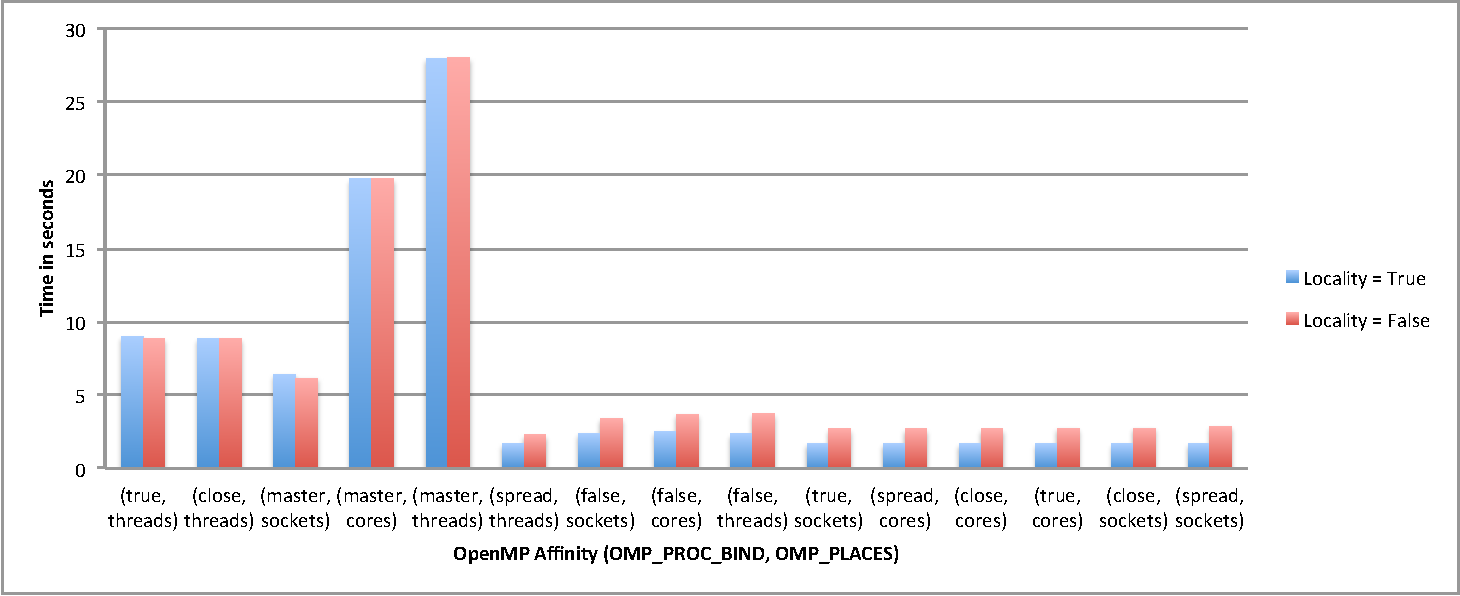
\includegraphics[height=0.4\textwidth, width=0.95\textwidth]{./Images/20Perf.pdf}
       \caption{Performance with 20 OpenMP threads on a two POWER8 socket system for the two versions of the Jacobi program.}
       \label{fig:20th}
\end{figure}
%
\begin{figure}[H]
  \centering
  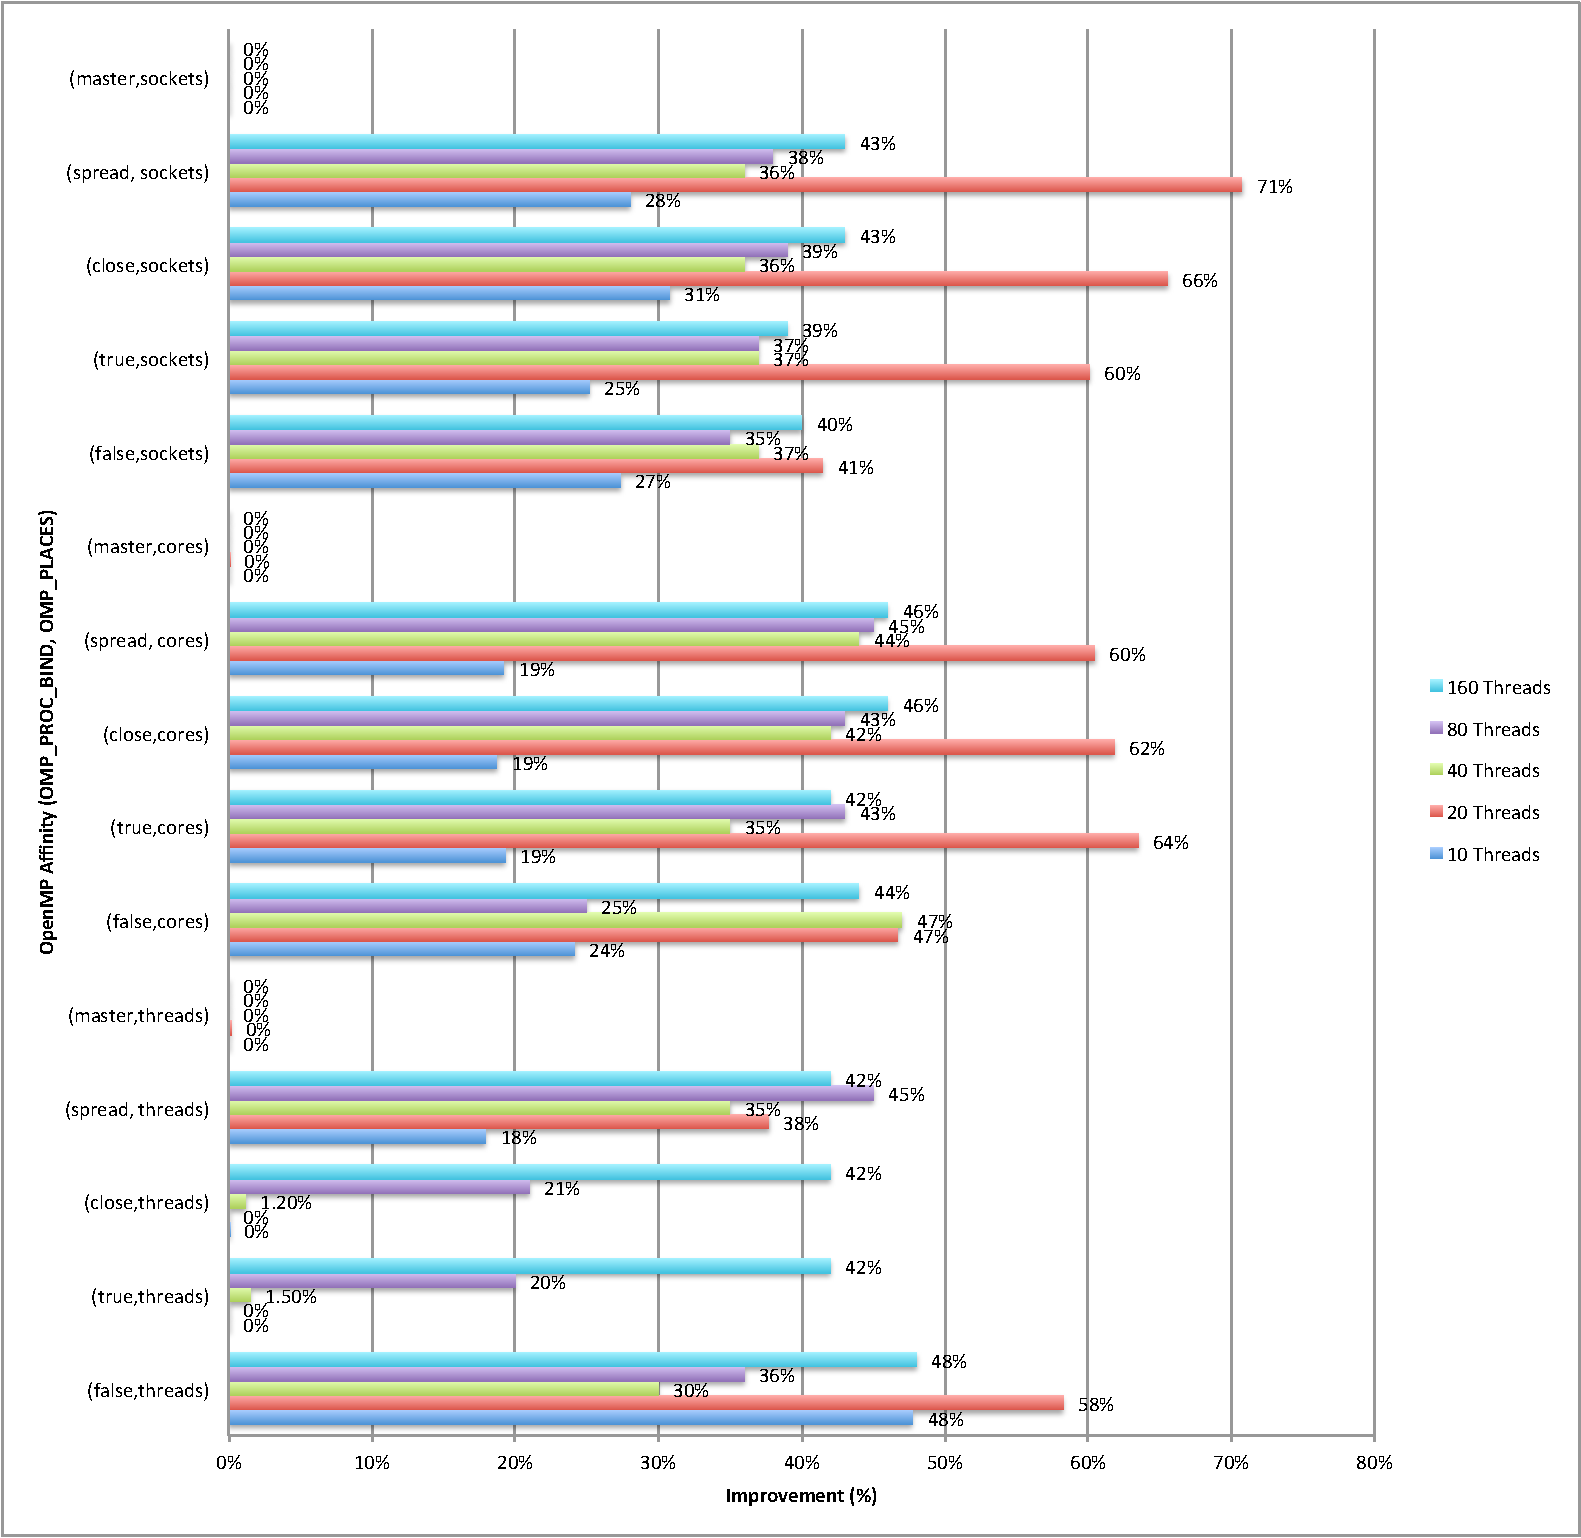
\includegraphics[height=1.2\textwidth, width=0.95\textwidth]{./Images/ImpAllV.pdf}
       \caption{Comparing Performance Improvement between the two version of the Jacobi program using 
       different number of OpenMP threads and thread affinity settings on a two POWER8 socket system}
       \label{fig:imp}
\end{figure}


In the \textit{(spread, sockets)} and \textit{(close, sockets)} configuration threads are spread across sockets but may be mapped to hardware threads running on same core. We observed that the \textit{(true, threads)} configuration is equivalent to the \textit{(close,threads)} according to the GCC OpenMP runtime thread mappings.
For all OpenMP affinity settings  with OMP\_PROC\_BIND set to false, threads can migrate and are not bound to a specific thread, core or socket. This migration makes it less impactful on the data placement, but suffers from degraded performance.

From the above discussion it is clear that not all OpenMP Affinity configurations are equal, moreover currently it lacks the ability to specify affinity based on NUMA \textbf{and} NUCA domains of emerging architectures like POWER8. This is the first step in understanding the need for new OpenMP affinity features to successfully deploying OpenMP on POWER machines. %Need something more here. 

%
%Hardware Counter notes
Next we look at the hardware counters on the POWER8 system corresponding to the different configurations to explain the improvement we observed in Figure~\ref{fig:imp}.
We select the three cases of OpenMP Affinity tuple that represent the best, mid, and worst improvement as seen in Figure~\ref{fig:imp}. 
%the cases where we see more improvement for data locality on a given affinity setting 
 \begin{figure}[h!]
  \centering
  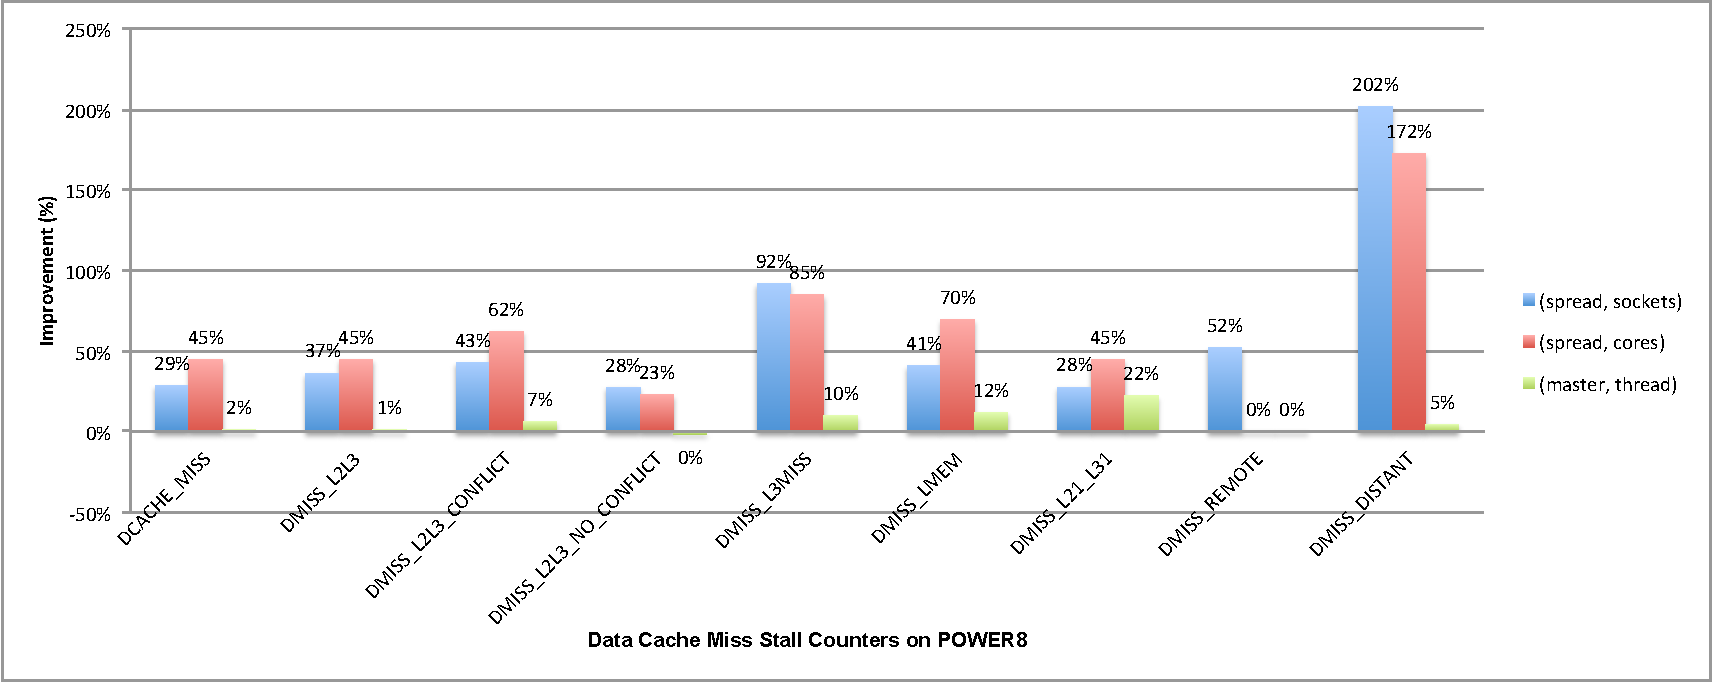
\includegraphics[height=0.4\textwidth, width=0.95\textwidth]{./Images/HW.pdf}
       \caption{Comparing Hardware Counter Change}
       \label{fig:HW}
\end{figure}
Selected cases are \textit{(spread, sockets)},  \textit{(spread, cores)}, and \textit{(master, thread)}. 
For these cases we record the hardware counters for the locality aware and locality unaware versions and calculate the improvement as the value of their difference as a percentage of the value of the locality unaware hardware counter value. 
From Figure~\ref{fig:HW} we see that the two hardware counters that show the effects of data locality the most are DMISS\_DISTANT, DMISS\_L3MISS.
We would have expected to see more significant variation in the value of DMISS\_REMOTE, but we found that in some cases, these remote accesses can be cached.
For example, the case of \textit{(spread, sockets)} has better DMISS\_REMOTE improvement than  \textit{(spread, cores)} which is counterintuitive. 
This is because in \textit{(spread, sockets)} some threads (not all) are running on the same core sharing local cache lines for (L1, L2) and thus taking advantage of cache reuse for remote data access. 
This can also be seen by the significant improvement in DMISS\_DISTANT which quantifies the stalls by L1 reloads from distant interventions and memory. The improvements we see in \textit{(spread, cores)} are more due to DMISS\_L21\_L31, which shows a better utilization of the L2/L3 cache as this hardware counter measures the stall cycles by Dcache miss which are resolved on chip. 
In the case of  \textit{(spread, cores)} we are effectively increasing the amount of 
L2 cache available to each OpenMP thread, as each thread has access to its own L2 cache on a given core. 
For the \textit{(master, thread)} case, there is very little improvement in the memory subsystem utilization as everything is running on the same thread (or CPU id) and the most of the data is local to the socket. In this case the data-locality version does not make any difference because all the threads are time-sharing the same hardware thread. This is also true for the case  \textit{(close, threads)} where
 we don't see improvements on the data locality aware version since data is local to the threads. POWER8 provides these unique set of hardware counters to distinguish OpenMP configurations that have less useless cycles on the memory sub-system. Specifically, DMISS\_REMOTE and, more importantly, DMISS\_DISTANT are key in identifying if the program suffers from bad data locality as indicated in Figure~\ref{fig:imp}.
%For example, from the data collected for 20 OpenMP threads \textit{(spread, threads)},  \textit{(close, cores)}, \textit{(true, cores)},  \textit{(close, sockets)}, \textit{(spread, sockets)} have similar high speed-ups but the PM\_CMPLU\_STALL\_DMISS\_L2L3 is least in the \textit{(spread, sockets)} configuration. 


 

\section{Related Work}
\label{sec:related}
%Thread placement and migration
Thread placement can be judiciously managed by runtime systems by monitoring hardware counters and maximizing total local memory accesses across all threads for an OpenMP region~\cite{Su:2011} by factoring in the critical path. Other strategies include examining the communication patterns to discover different thread placement strategies, so that they may benefit from shared caches, through either brute force or heuristic methods~\cite{5581451}. 

%Data placement, migration, and replication
Solaris, Windows and Linux use the first-touch policy by default. To address applications that are not suited for the first-touch policy, that is, where the access patterns are not the same throughout the life of the threads~\cite{Terboven:2008} developed the next-touch policy where the data is marked to be moved to the vicinity (core or node) of the next thread accessing the data. Unfortunately this policy comes with its own set of performance issues and has not been widely accepted for scalability reasons even with improvements~\cite{Goglin:2009} such as kernel based next-touch strategy which migrates only selected pages. For many systems, it may be prudent to replicate data, instead of migrating it. This was demonstrated in~\cite{Bull02} where the cost of replication was less than migration, through they conceded that some combination of replication and migration can achieve comparable performance. Studies in~\cite{Norden:2008} focus on geographical locality for applications with dynamic access patterns and shows that migration can lead to better performance and the need for directive level migration-on-next-touch support for OpenMP applications. Data mapping suggestions and page placement for different architectures has been explored in~\cite{Smeds2003,Marathe:2006}. Up to 20\% improvement in the benchmarks��s performance was observed~\cite{Marathe:2006} when page placement was directed via feedback about the memory accesses and dynamic memory allocation. Though this study is specific to Itanium-2 general principles are applicable to all ccNUMA systems.

Dynamic thread distribution as studied by~\cite{Matthias:2009} allows multi-level thread scheduler combined with a NUMA-aware memory manager to provide hints by the runtime to be able to either re-distribute threads or migrate data upon next-touch. For providing better ccNUMA locality of data, dynamic distribution of tasks through locality aware queuing software has shown promise~\cite{DBLP:journals2011}.




% An example of a floating figure using the graphicx package.
% Note that \label must occur AFTER (or within) \caption.
% For figures, \caption should occur after the \includegraphics.
% Note that IEEEtran v1.7 and later has special internal code that
% is designed to preserve the operation of \label within \caption
% even when the captionsoff option is in effect. However, because
% of issues like this, it may be the safest practice to put all your
% \label just after \caption rather than within \caption{}.
%
% Reminder: the "draftcls" or "draftclsnofoot", not "draft", class
% option should be used if it is desired that the figures are to be
% displayed while in draft mode.
%
%\begin{figure}[!t]
%\centering
%\includegraphics[width=2.5in]{myfigure}
% where an .eps filename suffix will be assumed under latex, 
% and a .pdf suffix will be assumed for pdflatex; or what has been declared
% via \DeclareGraphicsExtensions.
%\caption{Simulation Results}
%\label{fig_sim}
%\end{figure}

% Note that IEEE typically puts floats only at the top, even when this
% results in a large percentage of a column being occupied by floats.


% An example of a double column floating figure using two subfigures.
% (The subfig.sty package must be loaded for this to work.)
% The subfigure \label commands are set within each subfloat command, the
% \label for the overall figure must come after \caption.
% \hfil must be used as a separator to get equal spacing.
% The subfigure.sty package works much the same way, except \subfigure is
% used instead of \subfloat.
%
%\begin{figure*}[!t]
%\centerline{\subfloat[Case I]\includegraphics[width=2.5in]{subfigcase1}%
%\label{fig_first_case}}
%\hfil
%\subfloat[Case II]{\includegraphics[width=2.5in]{subfigcase2}%
%\label{fig_second_case}}}
%\caption{Simulation results}
%\label{fig_sim}
%\end{figure*}
%
% Note that often IEEE papers with subfigures do not employ subfigure
% captions (using the optional argument to \subfloat), but instead will
% reference/describe all of them (a), (b), etc., within the main caption.


% An example of a floating table. Note that, for IEEE style tables, the 
% \caption command should come BEFORE the table. Table text will default to
% \footnotesize as IEEE normally uses this smaller font for tables.
% The \label must come after \caption as always.
%
%\begin{table}[!t]
%% increase table row spacing, adjust to taste
%\renewcommand{\arraystretch}{1.3}
% if using array.sty, it might be a good idea to tweak the value of
% \extrarowheight as needed to properly center the text within the cells
%\caption{An Example of a Table}
%\label{table_example}
%\centering
%% Some packages, such as MDW tools, offer better commands for making tables
%% than the plain LaTeX2e tabular which is used here.
%\begin{tabular}{|c||c|}
%\hline
%One & Two\\
%\hline
%Three & Four\\
%\hline
%\end{tabular}
%\end{table}


% Note that IEEE does not put floats in the very first column - or typically
% anywhere on the first page for that matter. Also, in-text middle ("here")
% positioning is not used. Most IEEE journals/conferences use top floats
% exclusively. Note that, LaTeX2e, unlike IEEE journals/conferences, places
% footnotes above bottom floats. This can be corrected via the \fnbelowfloat
% command of the stfloats package.




\section{Conclusions and Future Work}
\label{sec:conclusion}
In this paper we evaluated OpenMP affinity support as well as memory placement on the POWER8 architecture. 
Data locality and affinity are key concepts to exploit the compute and memory capabilities to achieve good performance by minimizing data motion across NUMA domains. 
The main contribution of this paper is to evaluate current affinity features of OpenMP 4.0 on the POWER8 processors, and on how to measure its effect on data locality on a system with two P8 sockets. 
%What we observe from the experiments is that the effect of data placement and data locality is dependent on how threads are mapped to the architectures. 
In some OpenMP affinity test cases, we show that the POWER8 architecture, using its NUCA L3 caches, can hide the cost of accessing remote memory (as shown in the experiment \textit{(spread, cores)} when running a thread per core since it maximizes local caches that are available per thread. 
In other cases, when threads share some of the cores, there is a benefit of cache reuse in the non-shared L2 and L1 caches thus improving data locality in the application.
 In this paper we show that optimizing an application for data locality, the improvements will depend on the kind of affinity used. 

Future version of OpenMP affinity model need to support better the concept of NUMA domains. 
This can be made possible by supporting another \textit{place} option called \textit{Numa} can be added to OpenMP 5.0 via the \emph{OMP\_PLACES} ICV so that threads can be mapped more efficiently to NUMA domains. Although the same effect can be achieved by using OS supported bindings (\textit{taskset} on linux platforms), it is not a portable mechanism. By introducing the support of NUMA domains at the OpenMP level, we can keep the implementation details opaque from the programmer while providing a portable solution across all architectures.

Another type of extensions is to integrate the concept of OMP\_PLACES with the OpenMP target directive and device\_num. Our next step would be to explore ways of mapping OpenMP \emph{target} and \emph{target data} 
regions to NUMA domains to control data and thread placement.

% conference papers do not normally have an appendix

% use section* for acknowledgement
\section*{Acknowledgment}
\label{sec:ack}
This material is based upon work supported by the U.S. Department of Energy, Office of Science
under the Advanced Scientific Computing Research (ASCR) program. This research used resources of 
the Oak Ridge Leadership Computing Facility at the Oak Ridge National Laboratory, 
which is supported by the Office of Science of the U.S. Department of Energy under 
Contract No. DE-AC05-00OR22725.


The authors would like to thank...
more thanks here


% trigger a \newpage just before the given reference
% number - used to balance the columns on the last page
% adjust value as needed - may need to be readjusted if
% the document is modified later
%\IEEEtriggeratref{8}
% The "triggered" command can be changed if desired:
%\IEEEtriggercmd{\enlargethispage{-5in}}

% references section

% can use a bibliography generated by BibTeX as a .bbl file
% BibTeX documentation can be easily obtained at:
% http://www.ctan.org/tex-archive/biblio/bibtex/contrib/doc/
% The IEEEtran BibTeX style support page is at:
% http://www.michaelshell.org/tex/ieeetran/bibtex/
%\bibliographystyle{IEEEtran}
% argument is your BibTeX string definitions and bibliography database(s)
%\bibliography{IEEEabrv,../bib/paper}
%
% <OR> manually copy in the resultant .bbl file
% set second argument of \begin to the number of references
% (used to reserve space for the reference number labels box)
%\begin{thebibliography}{1}
%
%\bibitem{IEEEhowto:kopka}
%H.~Kopka and P.~W. Daly, \emph{A Guide to \LaTeX}, 3rd~ed.\hskip 1em plus
%  0.5em minus 0.4em\relax Harlow, England: Addison-Wesley, 1999.
%\end{thebibliography}

\bibliographystyle{IEEEtran}
\bibliography{references}



% that's all folks
\end{document}


